\chapter{Budowa bazy mobilnej}
\label{sec:robot}
\section{Dookólna platforma mobilna}
	\begin{figure}[H]
	\centering
	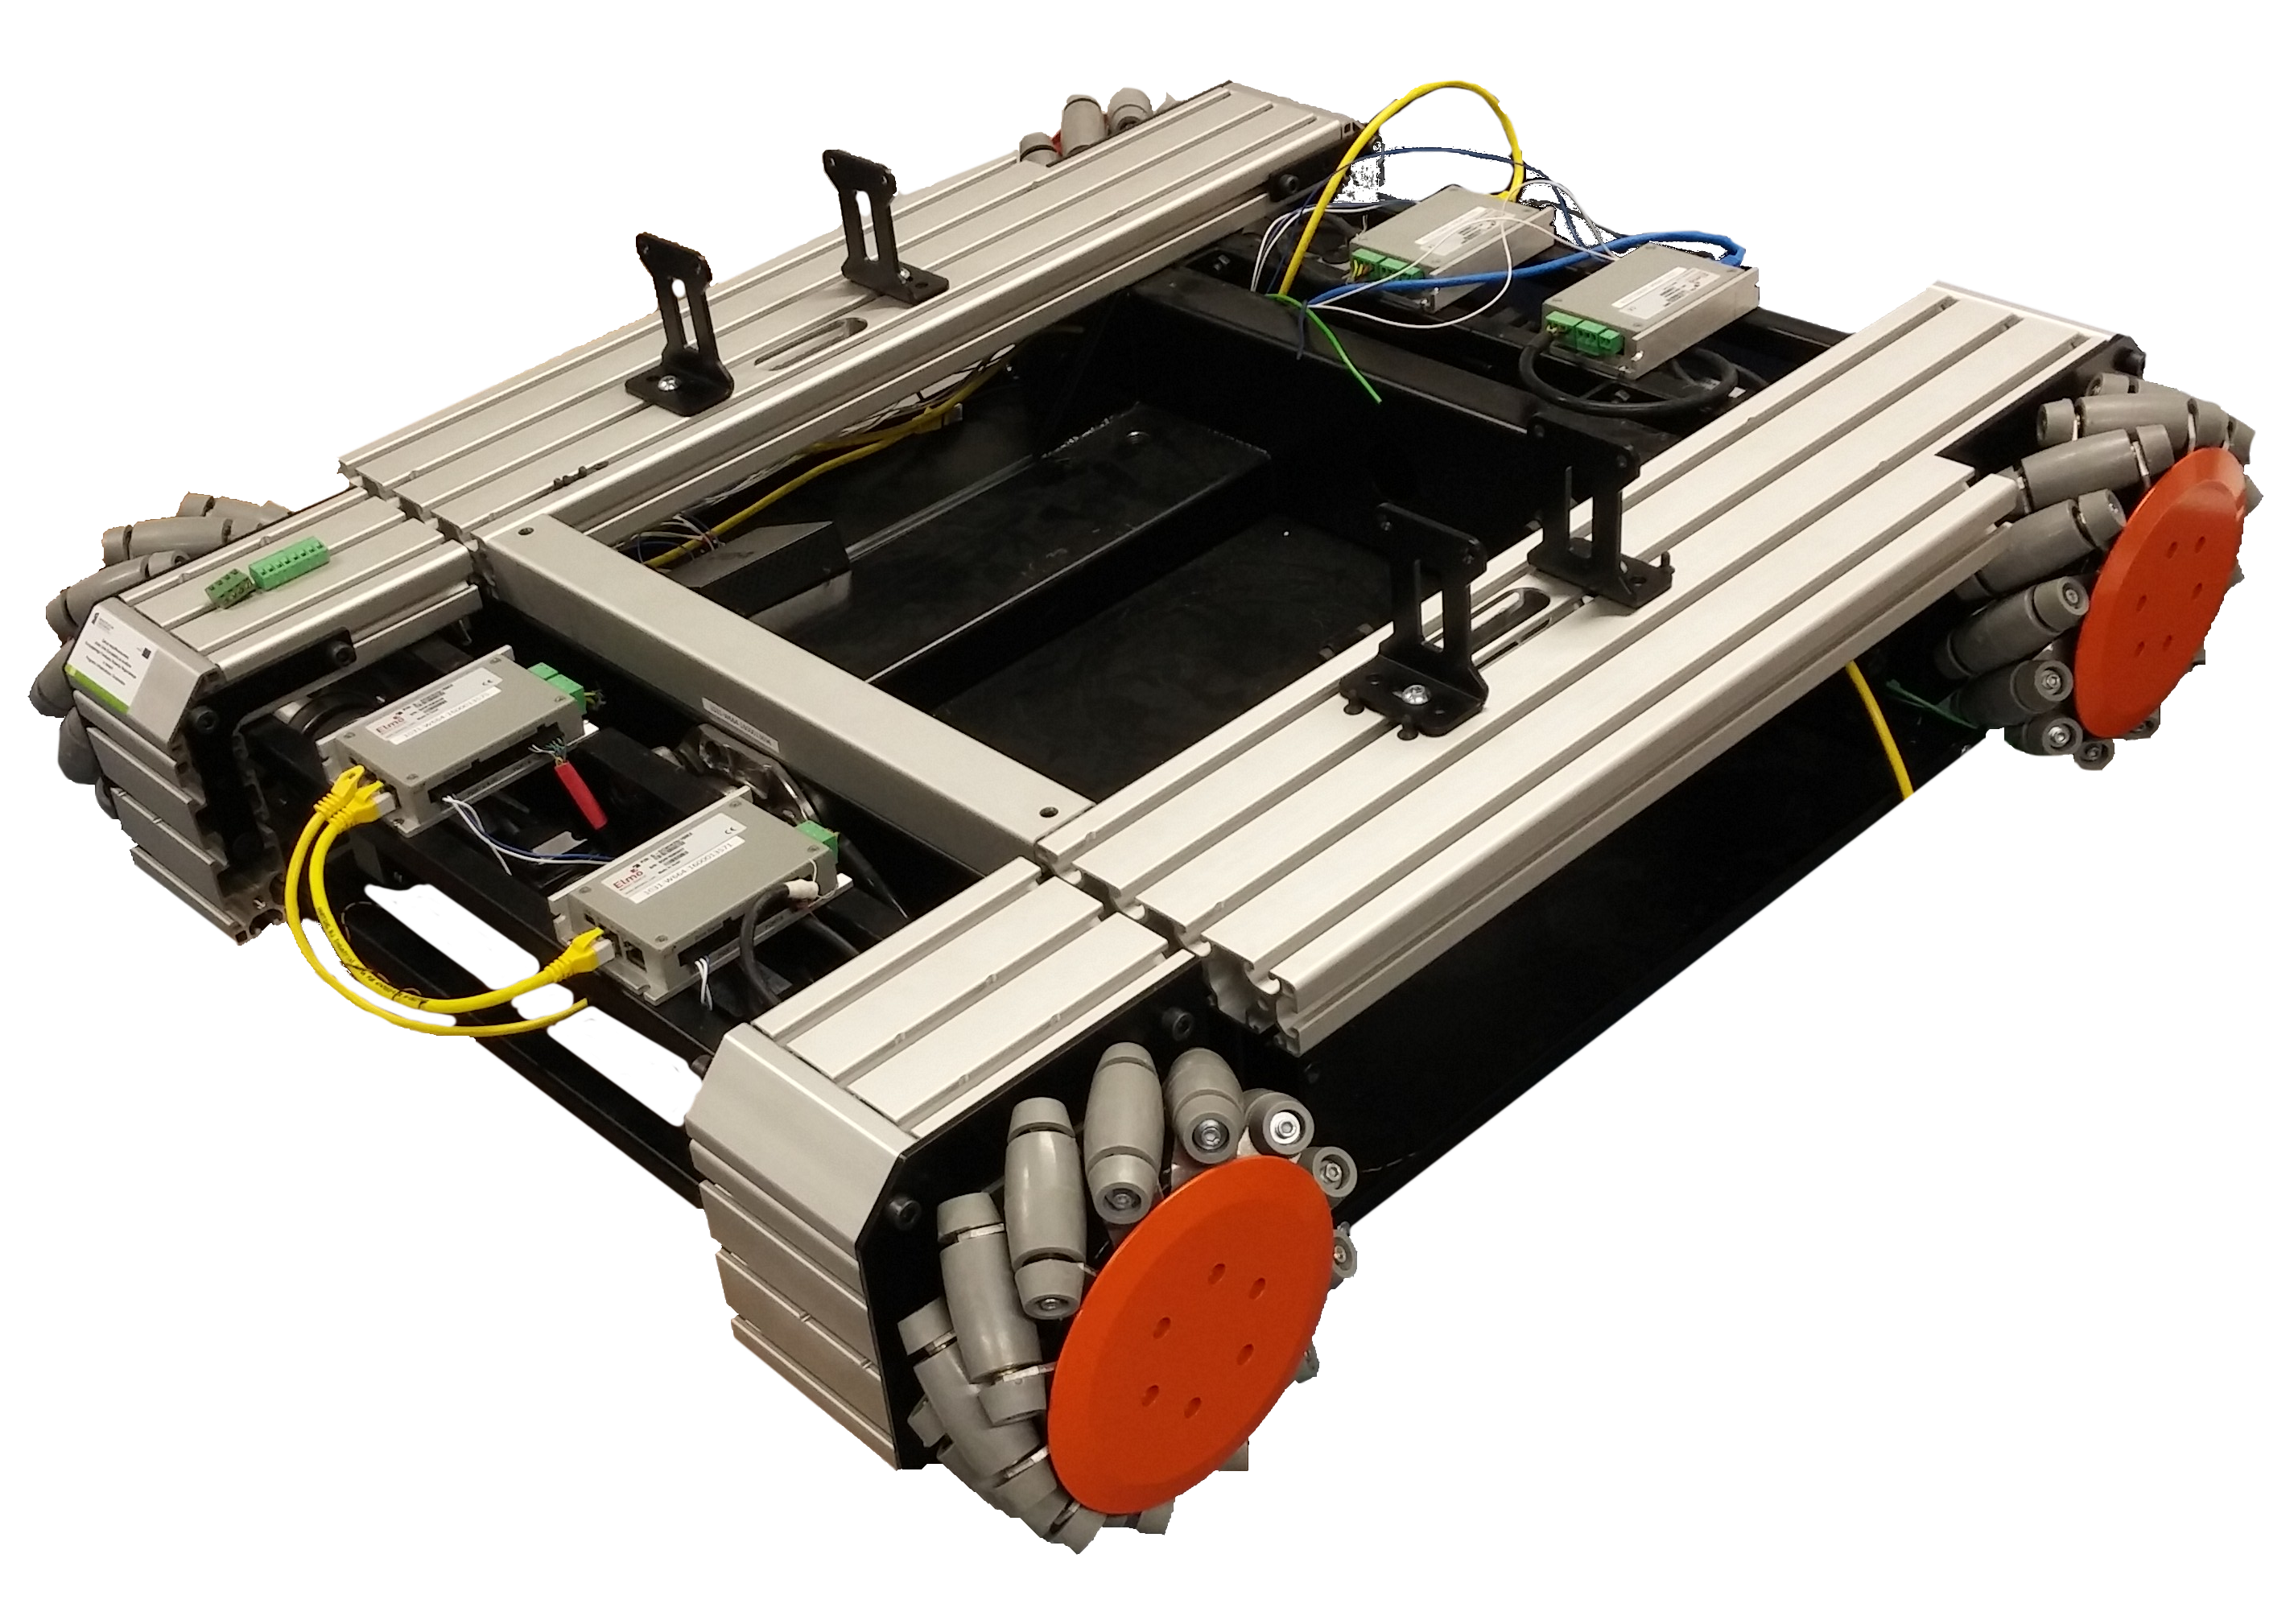
\includegraphics[width=0.8\textwidth]{graphics/base_photo.png}
	\caption{Dookólna baza mobilna na kołach szwedzkich.}
	\label{fig:base_photo}
	\end{figure} 

	Jest to duża, prostokątna baza dookólna poruszająca się na czterech kołach szwedzkich (rysunek \ref{fig:base_photo}).
	Koła są stałe, parami przytwierdzone do dwóch osi.
	Każde koło jest napędzane niezależnie przez podłączony bezpośrednio serwomotor, 
	zatem może mieć prędkość i kierunek obrotu niezależny od pozostałych kół.
	Każdy z serwomotorów ma także wbudowany enkoder, który zwraca aktualny kąt i prędkość obrotu.

	Jest to jeden z najpopularniejszych typów dookólnych platform mobilnych, mających zastosowanie także w innych robotach, jak na przykład Kuka Youbot (rysunek \ref{fig:kuka_youbot}).
	Należy zwrócić uwagę na charakterystyczne ustawienie kół, identyczne jak w opisywanej platformie na rysunku \ref{fig:base_photo}.
	
	Istnieją także roboty z trzema kołami szwedzkimi, w których koła rozstawione są na wierzchołkach trójkąta równobocznego.
	Pomimo prostszej budowy i takiej samej liczby stopni swobody, jak czterokołowa wersja, stabilność takiej konstrukcji jest gorsza \cite{extra_axis}.
	Ponieważ jest to robot transportowy, to stabilność odgrywa tu istotną rolę i czterokołowa konstrukcja jest wskazana.

	\begin{figure}[H]
	\centering
	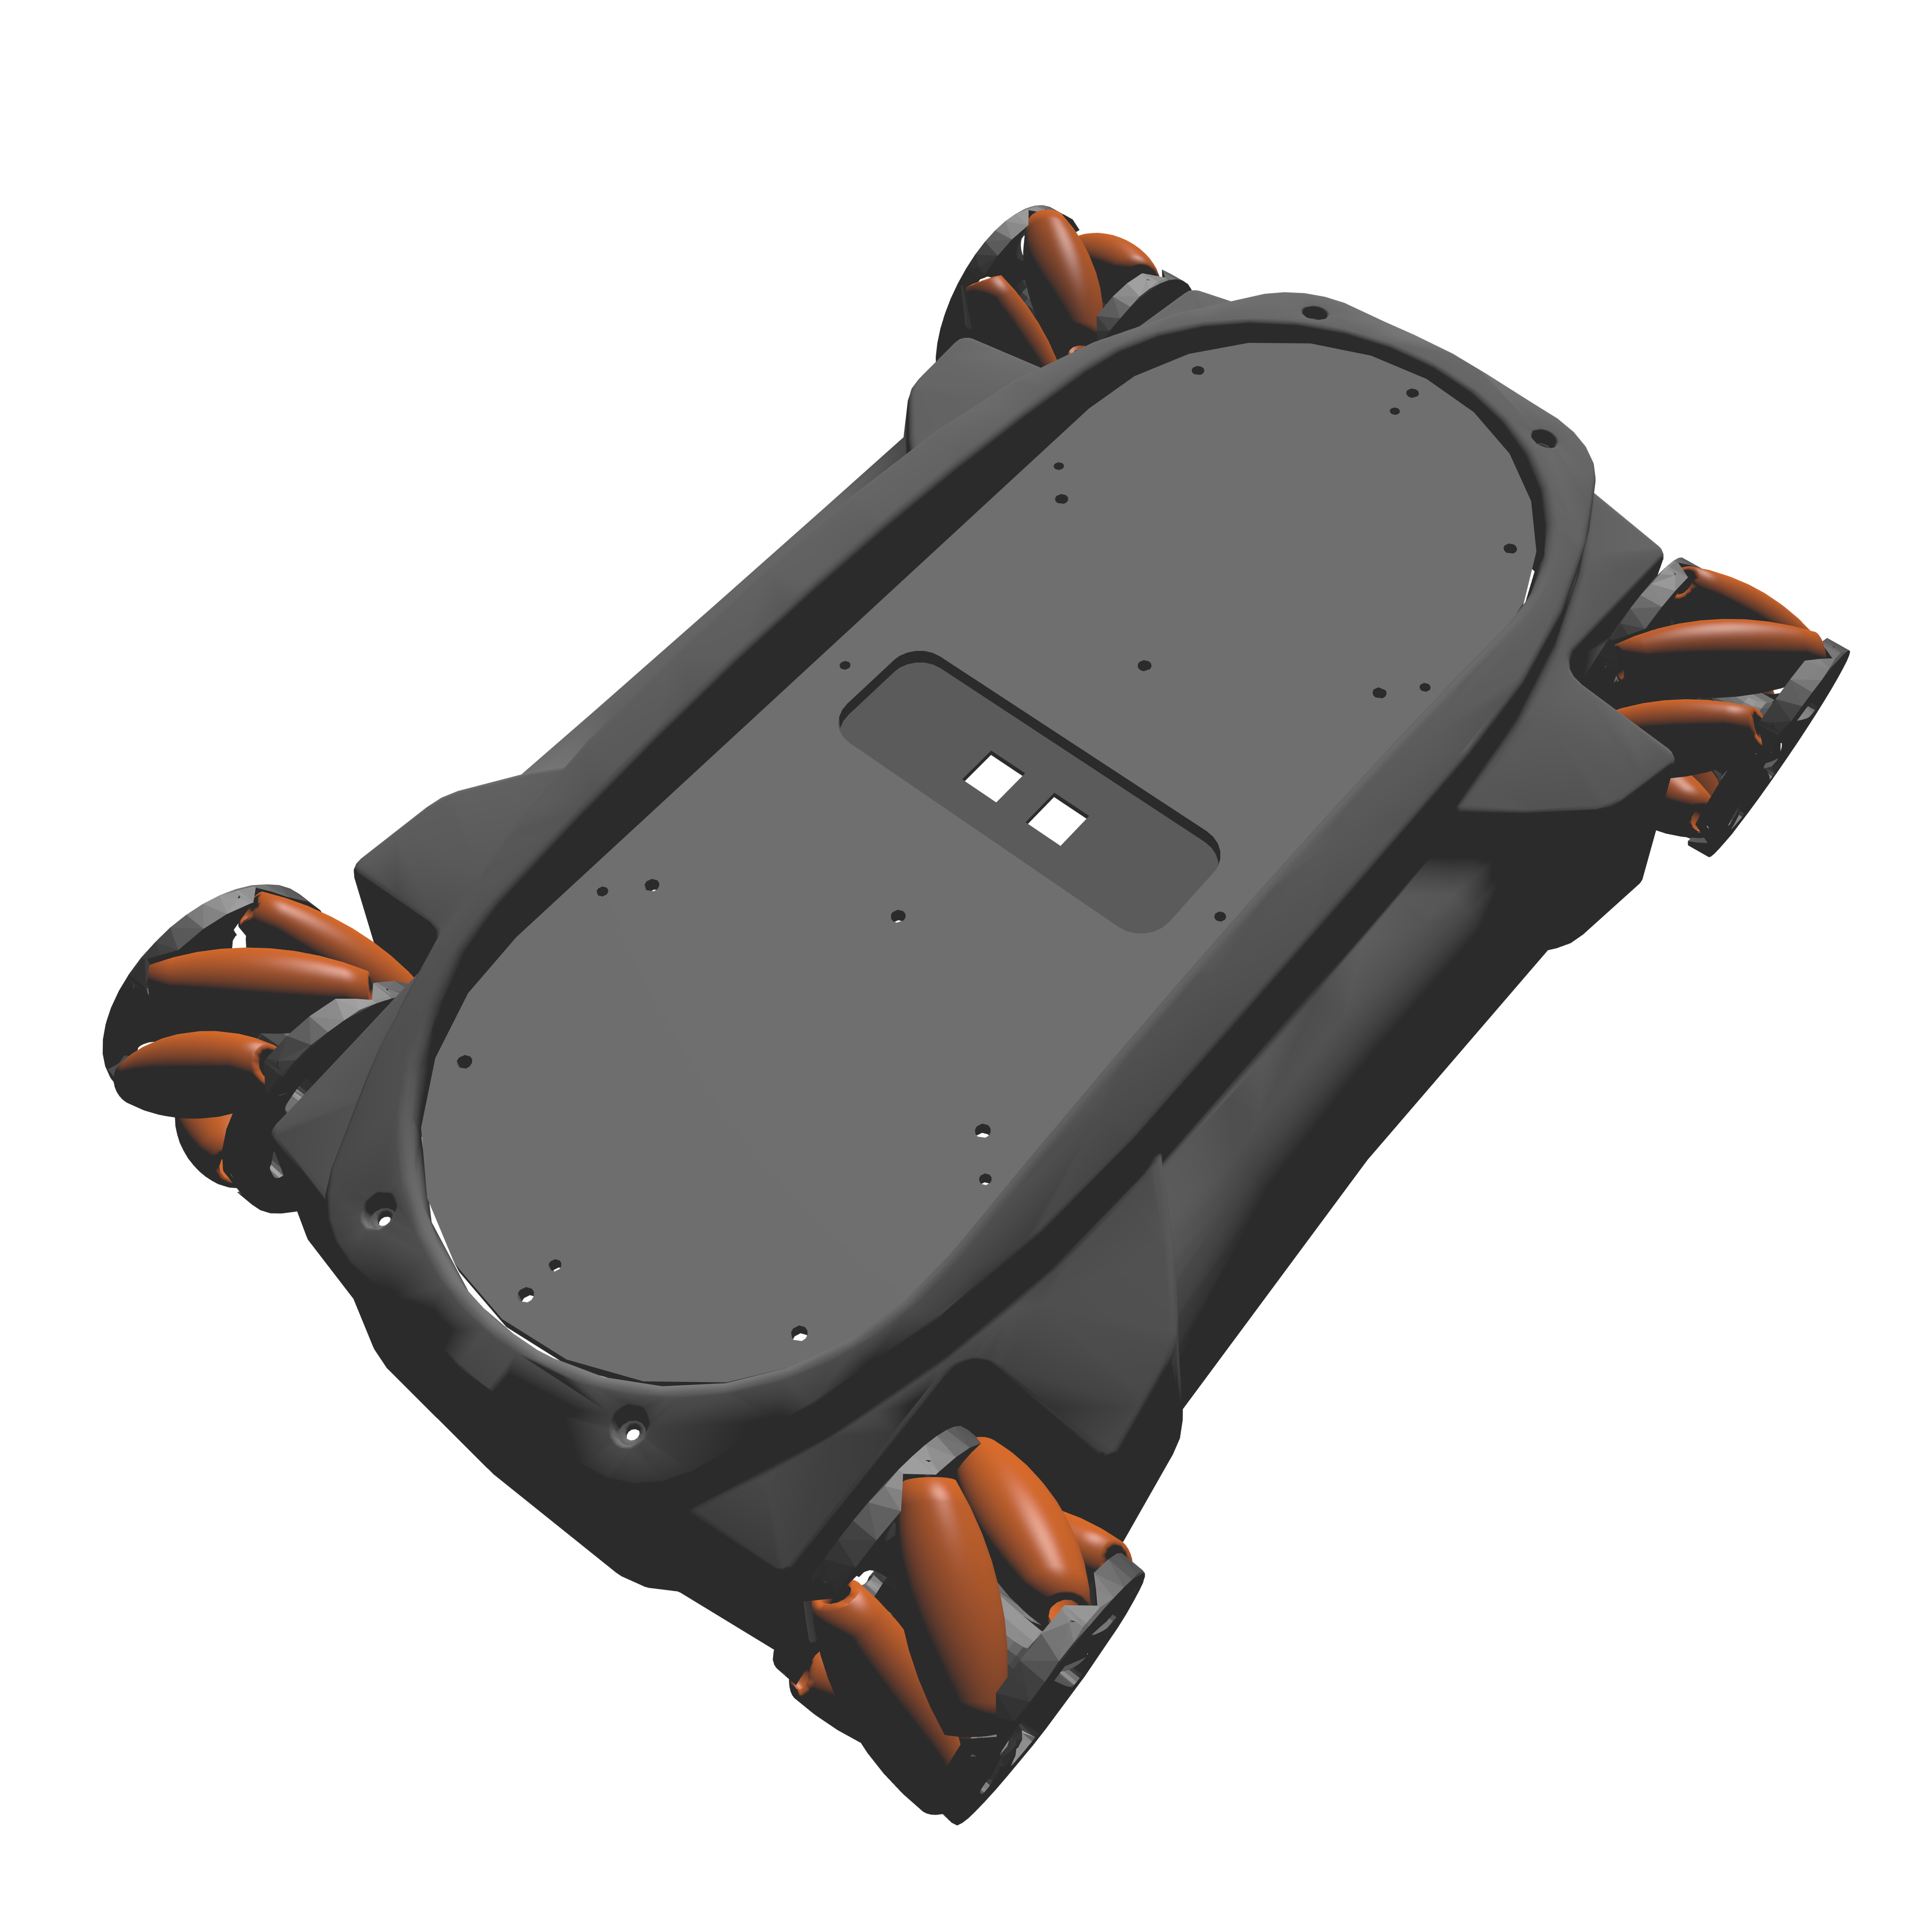
\includegraphics[width=0.5\textwidth]{graphics/kuka_youbot.png}
	\caption{Platforma robota Kuka Youbot \cite{kuka}.}
	\label{fig:kuka_youbot}
	\end{figure} 

	Odpowiedni obrót kół pozwala na jej ruch w dowolnym kierunku, niezależnym od orientacji robota, patrz rysunek \ref{fig:mecanum_dirs}.
	Jest możliwe także obracanie bazą, gdy ta porusza się w dowolnym kierunku, bądź stoi w miejscu.
	
	\begin{figure}[H]
	\centering
	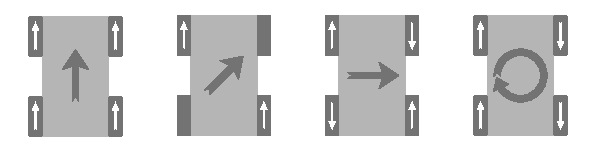
\includegraphics[width=0.8\textwidth]{graphics/mecanum_dirs.pdf}
	\caption{Podstawowe kierunki ruchu robota z napędem wielokierunkowym.}
	\label{fig:mecanum_dirs}
	\end{figure} 
	
	Przykładowo, poruszając tylko przeciwległymi kołami po przekątnej, robot będzie mógł poruszać się po skosie, bez zmiany orientacji bazy.
	A jeśli do tego dodać obrót kół drugiej przekątnej, w odwrotnym kierunku, wtedy pojazd zacznie się poruszać w bok, pomimo faktu, że koła nie są skrętne i 
	nie mogą ustawić się zgodnie z kierunkiem jazdy.
	Trasa, po której porusza się robot, przy stałej prędkości kół, zawsze jest łukiem okręgu. 
	W szczególnych przypadkach można uznać prostą za okrąg o nieskończonym promieniu, a punkt za okręg o zerowym. 
	Wynika to z faktu, że każdy obiekt, który ma jednostajną prędkość i stały kierunek w lokalnym układzie współrzędnych oraz stałą prędkość kątową, będzie się poruszał po łuku.
	Zależność promienia okręgu $R$ od prędkości liniowej $v$ i prędkości kątowej $\omega$, wyraża się wzorem $R = \frac{v}{\omega}$.

	Baza mobilna będzie podstawą dwuramiennego robota Velma, tworząc razem manipulator mobilny.
	Velma to dwuramienny robot, każde ramkę o 7 stopniach swobody, wyposażony w dwa chwytaki (patrz rysunek \ref{fig:velma}).
	Taka budowa wymaga szerokiej podstawy, aby zachować bezpieczną równowagę całości.
	Jeżdżąc na tej bazie, robot może się przemieszczać i obracać w dowolnym kierunku, aby zwiększyć swoją przestrzeń roboczą.

	\begin{figure}[H]
	\centering
	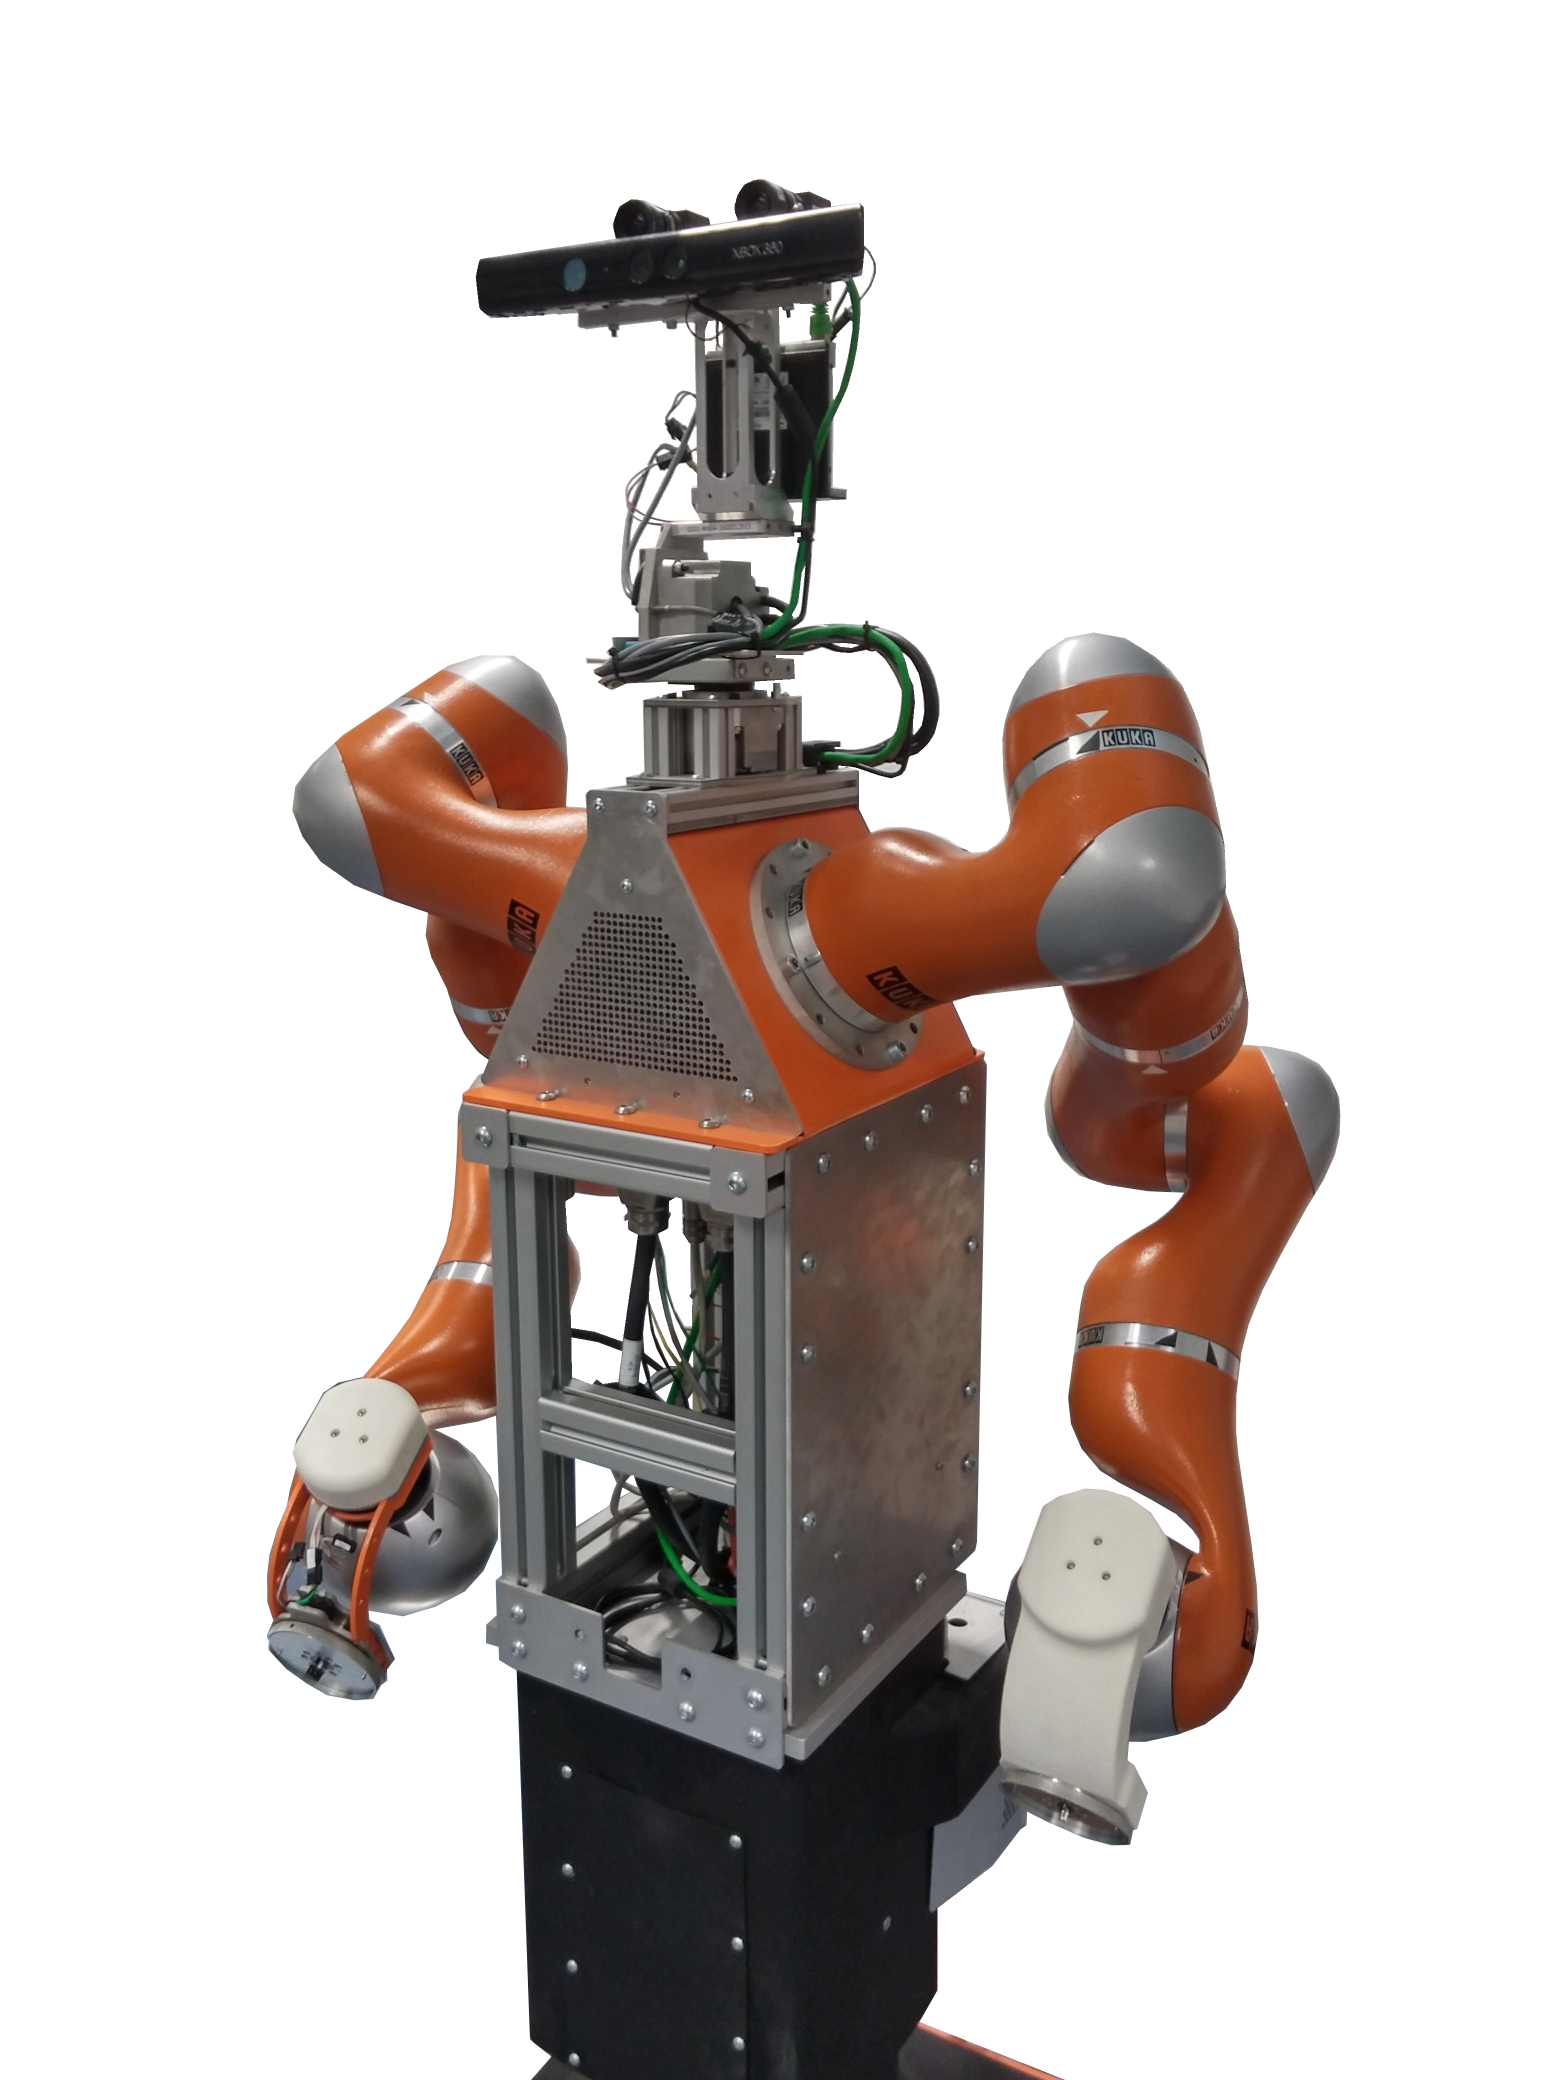
\includegraphics[width=0.5\textwidth]{graphics/velma.png}
	\caption{Dwuramienny robot Velma.}
	\label{fig:velma}
	\end{figure} 
	
	\begin{figure}[h]
		\centering
		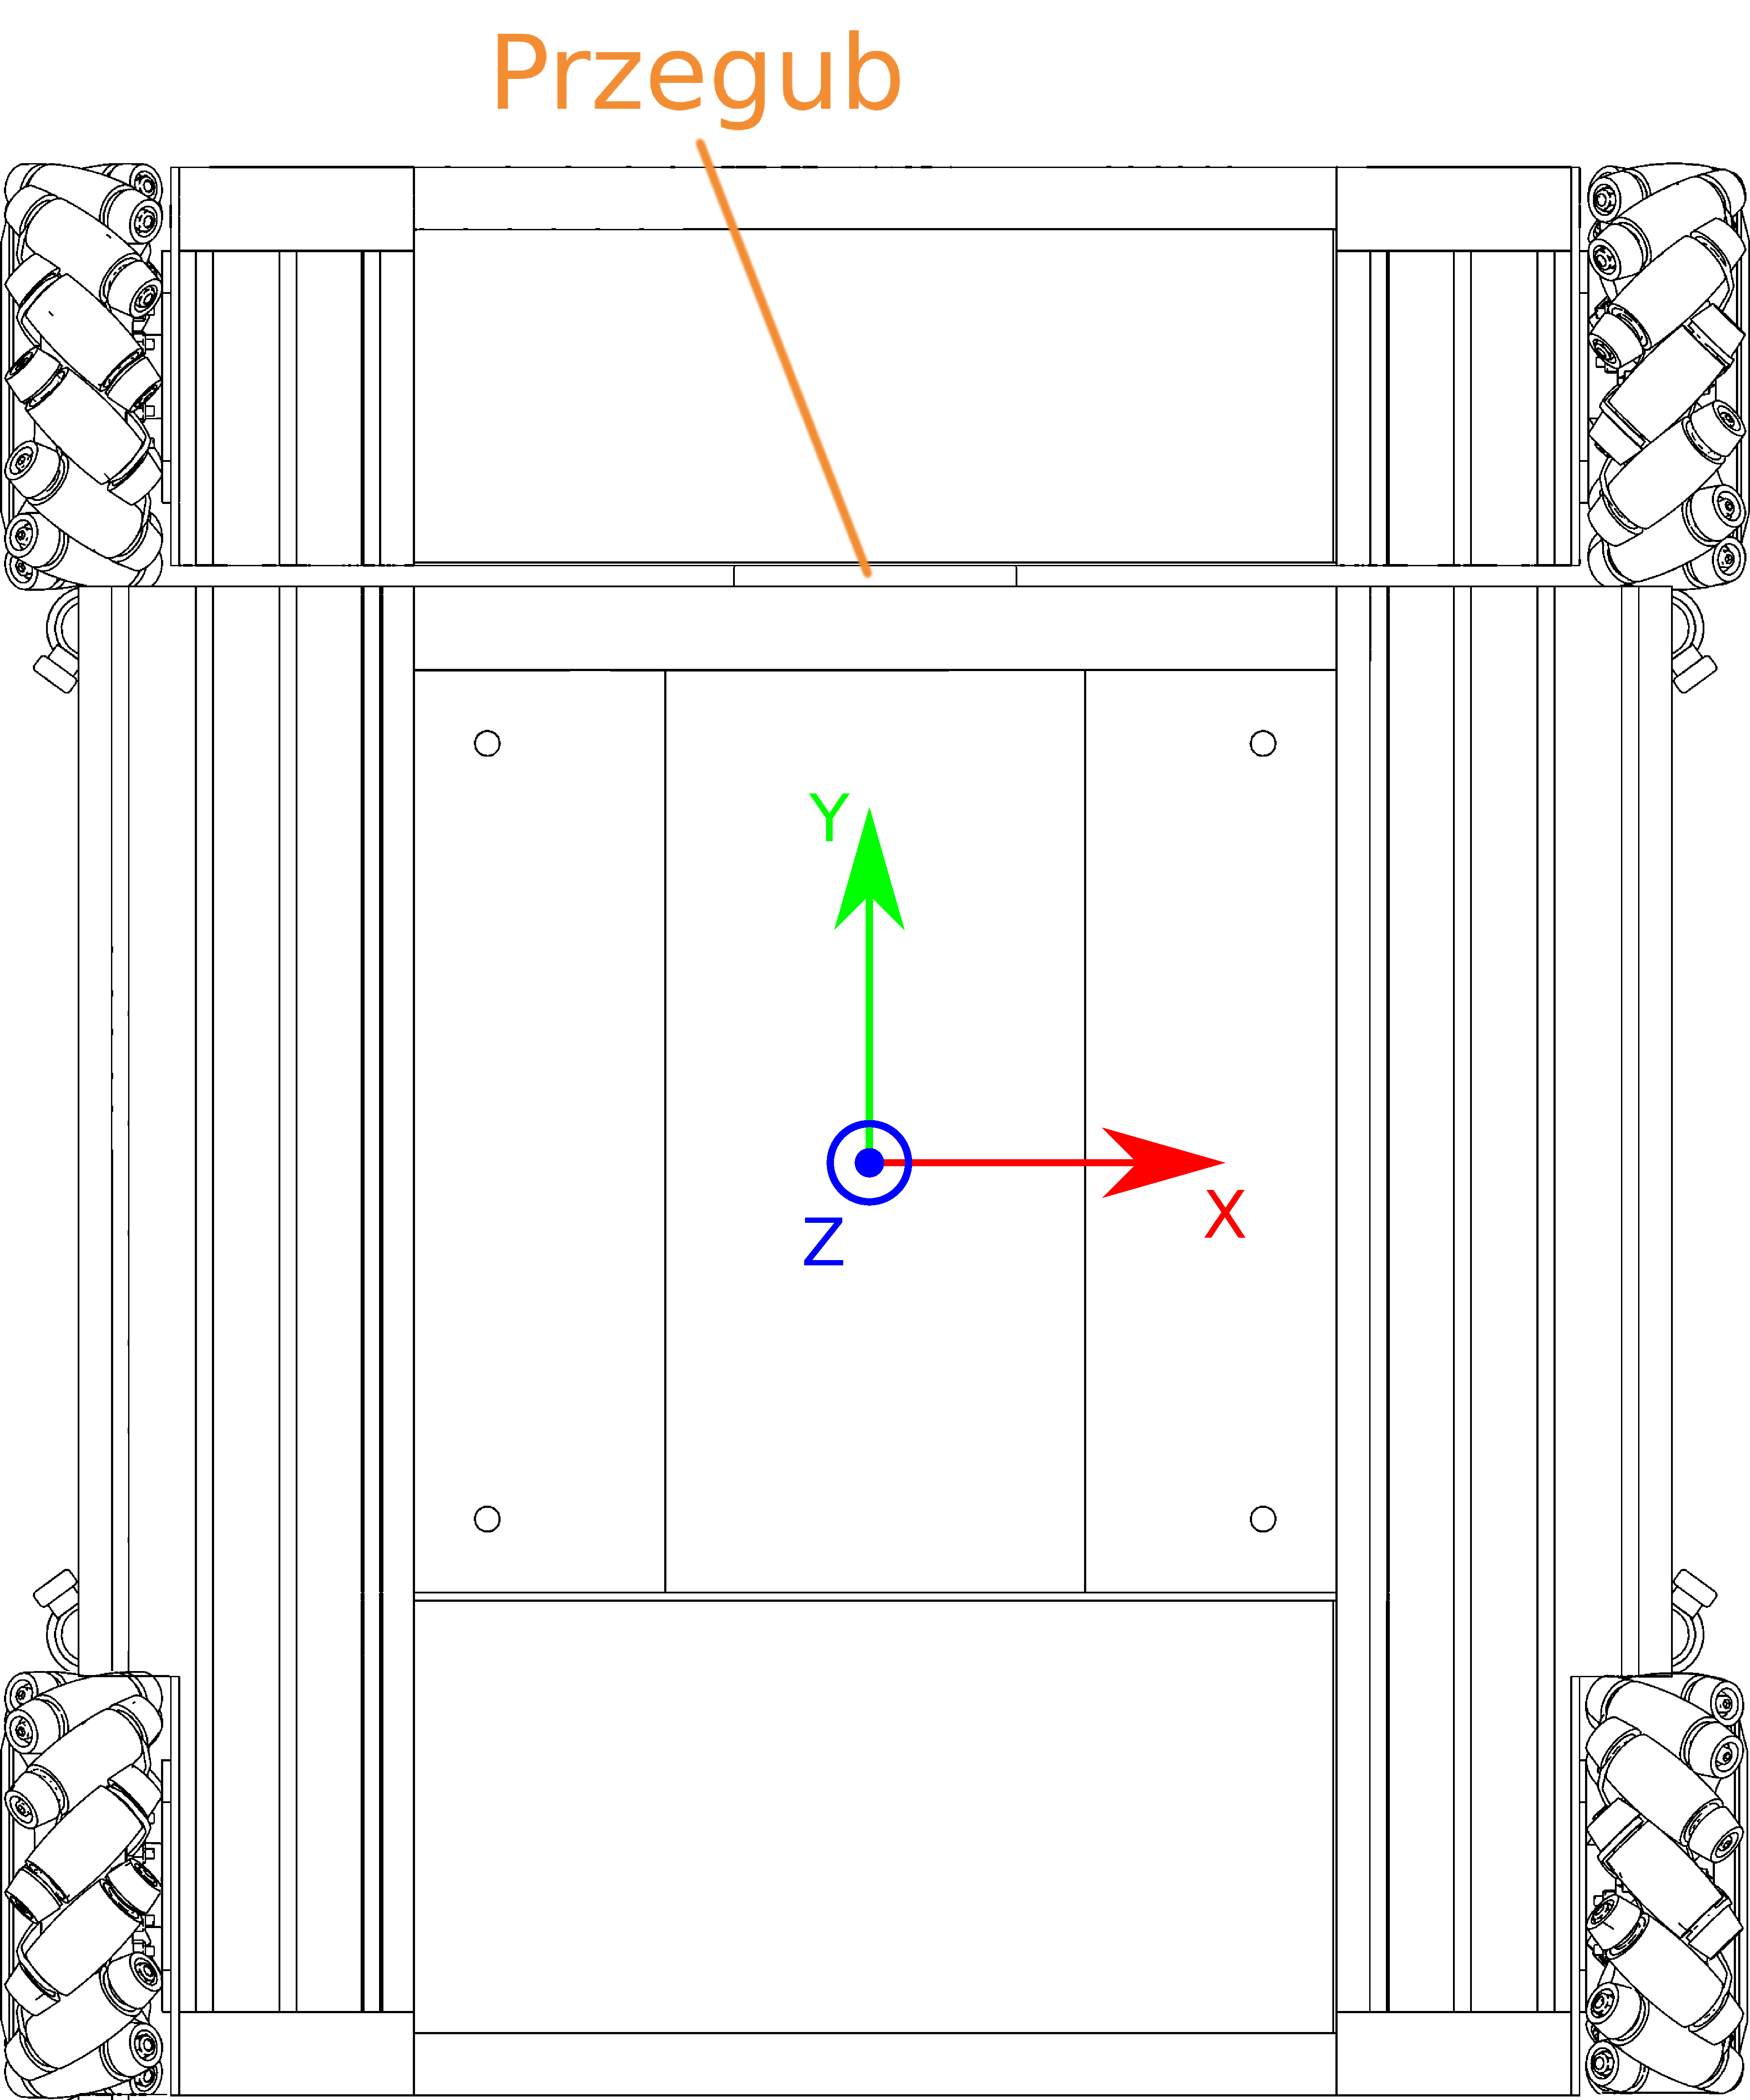
\includegraphics[width=0.8\textwidth]{graphics/base.pdf}
		\caption{Platforma mobilna w lokalnym układzie współrzędnych. Widoki: \textbf{a)} od góry, \textbf{b)} od prawej strony i \textbf{c)} od przodu. Przegub obrotowy łączy dwie części.}
		\label{fig:base_ortho}
	\end{figure} 

	Platforma mobilna jest niesymetrycznie podzielona na dwie części, przednią i tylną, w sposób pokazany na rysunku \ref{fig:base_ortho}.
	Przegub o jednym stopniu swobody jest jedynym łącznikiem pomiędzy tymi dwoma częściami.
	Zadaniem tego przegubu jest zmniejszanie wpływu nierówności podłoża na ruch bazy, aby każde koło zachowało stały kontakt z podłożem.
	Bez tego przegubu, ruch po nierównym terenie uniemożliwiałby sprawne sterowanie platformą na skutek nieprzewidywalnych zaników kontaktu kół z podłożem, powodując nieplanowane skręty.
	Takie zaniki kontaktu kół są niewykrywalne w bezpośredni sposób, jak to zostało opisane w \cite{boringbot}.

	Platforma ma kształt prostokąta o wymiarach $0,72\times0,76$ \si{\metre} (rysunek \ref{fig:base_dims} i tabela \ref{tab:dims}).
	Koła ustawione są na wierzchołkach tego prostokąta.

	Platforma może w trakcie hamowania poruszać się innym kierunku, niż tuż przed zatrzymaniem.
	Jest to spowodowane tym, że konstrukcja rolek powoduje poślizg platformy w kierunku obrotu rolki, mającej aktualnie kontakt z podłożem, a ten kierunek zależy od aktualnej
	orientacji bazy, nie od kierunku w jakim się porusza.
	Należy także uwzględnić inne cechy tego typu kół, jak nierówne tarcie poszczególnych rolek o powierzchnię \cite{braking}.

	Platforma ma 3 stopnie swobody. 
	\begin{itemize}
		\item Przesunięcie wzdłuż osi X.
		\item Przesunięcie wzdłuż osi Y.
		\item Obrót wokół osi prostopadłej do podłoża.
	\end{itemize}
	
	Kierunek osi X i Y (patrz rysunek \ref{fig:base_ortho}) układu jest zgodny z kierunkami przyjętymi w sterowaniu robotem.
	
	\begin{figure}[h]
		\centering
		\includegraphics[width=0.8\textwidth]{graphics/base_dims.pdf}
		\caption{Parametry geometryczne bazy i prędkości.}
		\label{fig:base_dims}
	\end{figure} 

	\begin{table}
		\centering
		\begin{tabular}{c c l}
		Oznaczenie & Wartość & Opis \\
		\hline
		$r$ & 0,1 \si{\metre} & Promień koła. \\
		$a$ & 0,76 \si{\metre} & Rozstaw kół na tej samej osi. \\
		$b$ & 0,72 \si{\metre} & Rozstaw osi. \\
		$\omega_i$ & & Prędkość kątowa $i$-tego koła. \\
		$v_x$ & & Składowa prędkości liniowej wzdłuż osi X. \\
		$v_y$ & & Składowa prędkości liniowej wzdłuż osi Y. \\
		$\omega_z$ & & Prędkość kątowa wokół osi Z, wektor skierowany w górę. \\
		\end{tabular}
		\caption{Parametry i zmienne modelu.}
		\label{tab:dims}
	\end{table}
	
\section{Koła szwedzkie}
	Koła szwedzkie, zwane także kołami Mecanum, to specjalne koła z dodatkowymi rolkami na obwodzie, ustawionymi pod kątem \ang{45} do osi koła.
	Rolki są pasywne i obracają się niezależnie od siebie. Każde koło ma 12 takich rolek (patrz rysunek \ref{fig:wheel}).
	W platformie ich osie ustawione są w ten sposób, że osie najwyższych, lub najniższych, rolek dwóch kół z tej samej strony platformy przecinają się pod kątem prostym.
	Innymi słowy, robot ma identycznie ustawione koła na przeciwległych wierzchołkach, i razem ustawione są w kształt litery \emph{X}, patrząc na nie z góry.
	Należy pamiętać, iż oś dolnej rolki jest prostopadła do osi górnej rolki.

	Koła zamontowane w platformie zostały wyprodukowane przez amerykańską firmę AndyMark \cite{andymark}.
	Koła mają średnice o okrągłej liczbie 8 cali, czyli 20,32 \si{\centi\metre} oraz grubość 7,41 \si{\centi\metre}.
	Każde koło waży 1,6 \si{\kilo\gram} i jest w stanie udźwignąć masę ok. 200 \si{\kilo\gram}.
	
	Każda rolka podzielona jest na 3 części (patrz rysunek \ref{fig:wheel}) w celu lepszego zamocowania na kole, każda część może obracać się niezależnie.
	Teoretycznie zatem każde koło ma 36 rolek, lecz nie ma to znaczenia z punktu widzenia symulacji.

	\begin{figure}[H]
	\centering
	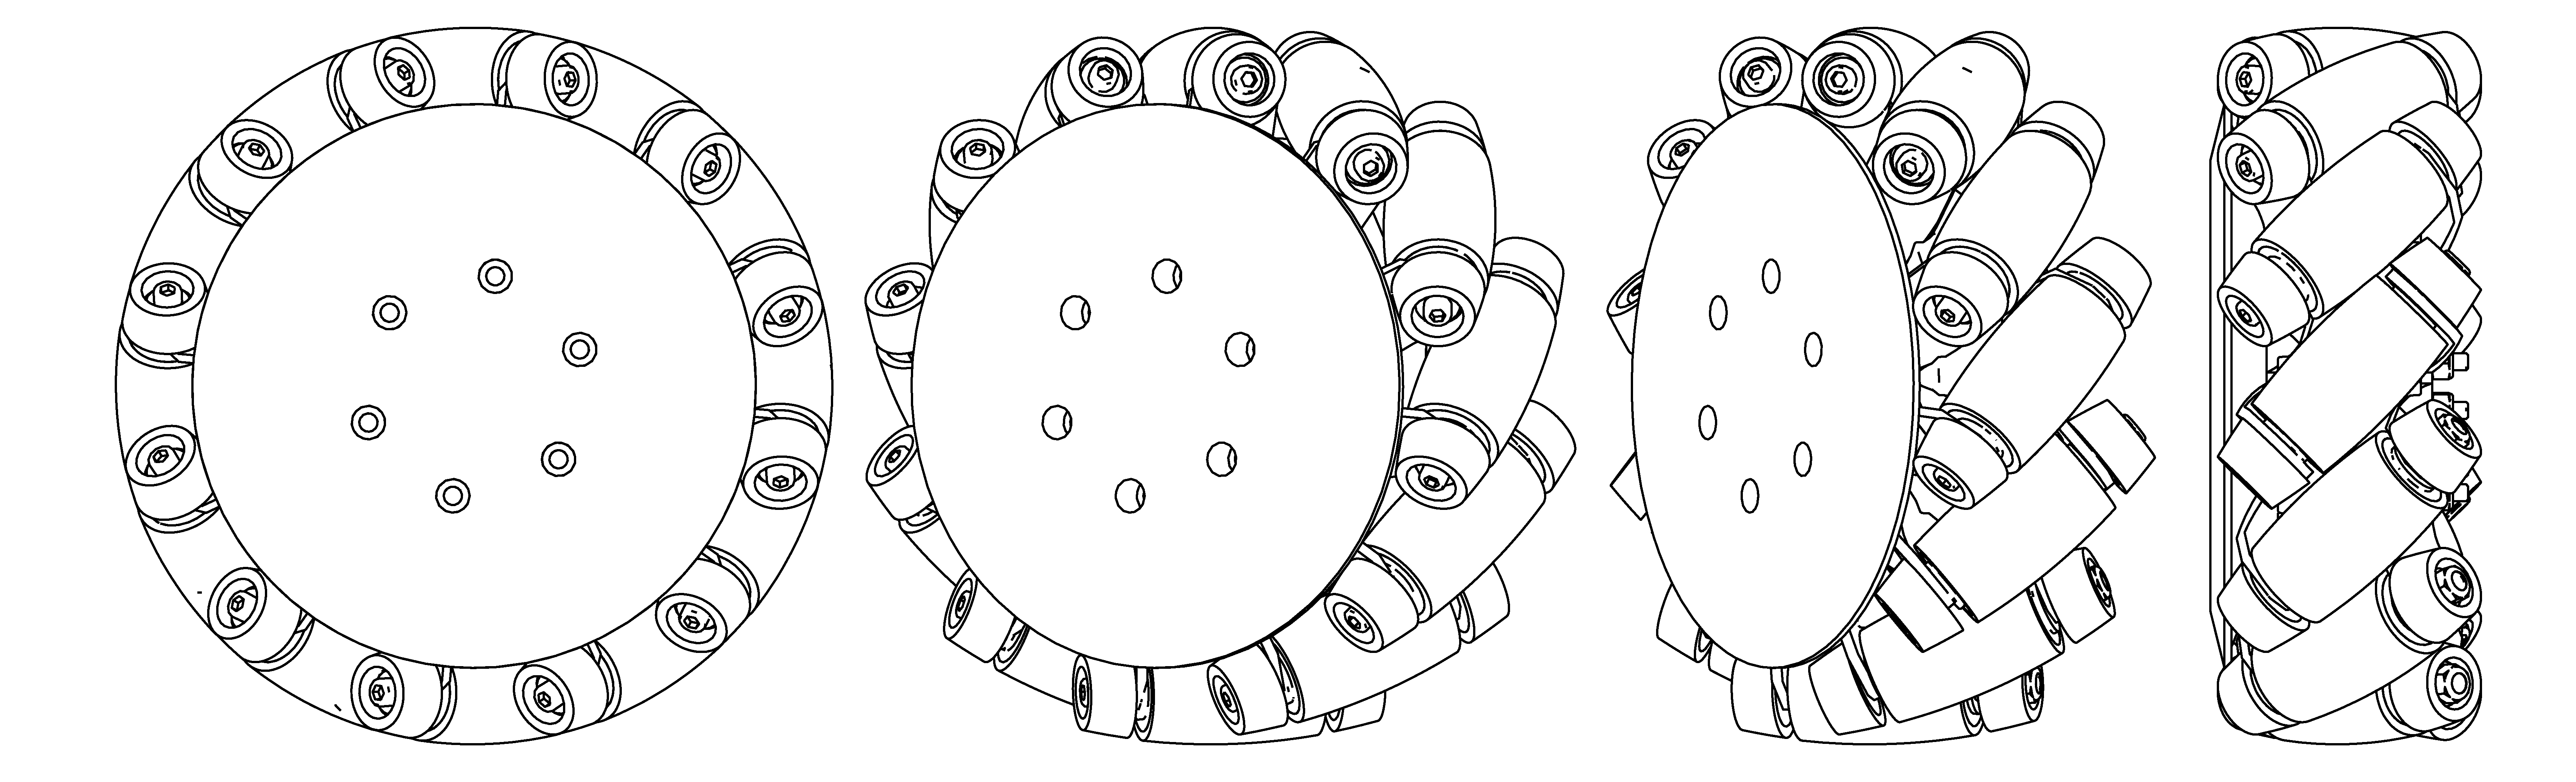
\includegraphics[width=\textwidth]{graphics/wheel.pdf}
	\caption{Widok 12 rolkowego koła szwedzkiego platformy wielokierunkowej.}
	\label{fig:wheel}
	\end{figure} 

	Każde koło ma 3 stopnie swobody \cite{kinematic_modeling}.
	\begin{itemize}
		\item Obrót koła w osi prostopadłej do płaszczyzny koła i przechodzącej przez jego środek.
		\item Obrót pojedynczych rolek.
		\item Poślizg rolki w miejscu styku rolki z podłożem.
	\end{itemize}

	Na podstawie rysunku \ref{fig:wheel} można zauważyć, że krzywizna rolki jest tak dobrana, aby punkt kontaktu rolki z podłożem w czasie obrotu koła płynnie przechodził na następną rolkę.
	Celem jest utrzymanie stałej odległości osi obrotu koła od płaszczyzny podłoża.
	Nie powinno być efektu przeskoku z jednej rolki na drugą, gdyż powoduje to nierówne tarcie, losowe poślizgi i nadmierne zużycie elementów wykonawczych.
	Kształt pojedynczej rolki jest wycinkiem paraboloidy, wzory opisujące kształt rolki są złożone.
	Zazwyczaj przybliża się taką rolkę wycinkiem torusa, w celu uproszczenia produkcji \cite{rollers}.

	Istnieją także koła o innej konstrukcji, złożone z wielu małych rolek, tak aby w każdym momencie więcej jak jedna rolka dotykała podłoża.
	Można także złożyć kilka tego typu kół obok siebie w jedno koło.
	Przydatne jest to dla robotów transportujących duże masy, gdyż zmniejsza to obciążenie pojedynczych rolek.
	Niestety, taka konstrukcja jest chroniona aktywnym patentem, więc pojedyncze koło, na które patent już wygasł, jest jedynym powszechnie używanym \cite{paletobot}.

	Pomimo skomplikowanej budowy, występują poślizgi rolek po powierzchni.
	Odległość osi obrotu koła od płaszczyzny podłoża nieznacznie zmienia się przy przenoszeniu obciążenia z rolki na rolkę, co przy dużych prędkościach powoduje drgania i jeszcze większe błędy wyznaczania pozycji na podstawie odometrii.

	\subsection{Opis ruchu}
		\label{sec:robot_movement}
		W zwykłym kole, dzięki sile tarcia, moment siły przekształcany jest na przyspieszenie w kierunku równoległym do podłoża i płaszczyzny koła.
		Dodatkowo wektory sił tarcia są równe we wszystkich kierunkach. To znaczy, koło będzie stawiało identyczny opór, niezależnie czy wektor siły będzie równoległy do osi koła, czy prostopadły do niego.
		
		Specjalne koło Mecanum nie powoduje sił tarcia w jednym z kierunków, oznaczonych jako $f_0$ nad rysunku \ref{fig:wheel_vectors}.
		Ten kierunek obrócony jest o 45° w stosunku do osi koła i jest zgodny z kierunkiem obrotu dolnej rolki.
		
		Po przyłożeniu momentu siły $M$, siła tarcia zadziała jedynie w kierunku prostopadłym do $f_0$, gdyż tylko w tym kierunku dolna rolka nie będzie w stanie się obracać.
		Czyli wypadkowy wektor siły $F$, nadający przyspieszenie kołu, również będzie zwrócony o kąt 45° w stosunku do osi obrotu rolki.
		
		Suma wektorów $F$ od wszystkich kół platformy nada jej odpowiedni kierunek ruchu.
		
		\begin{figure}[H]
			\centering
			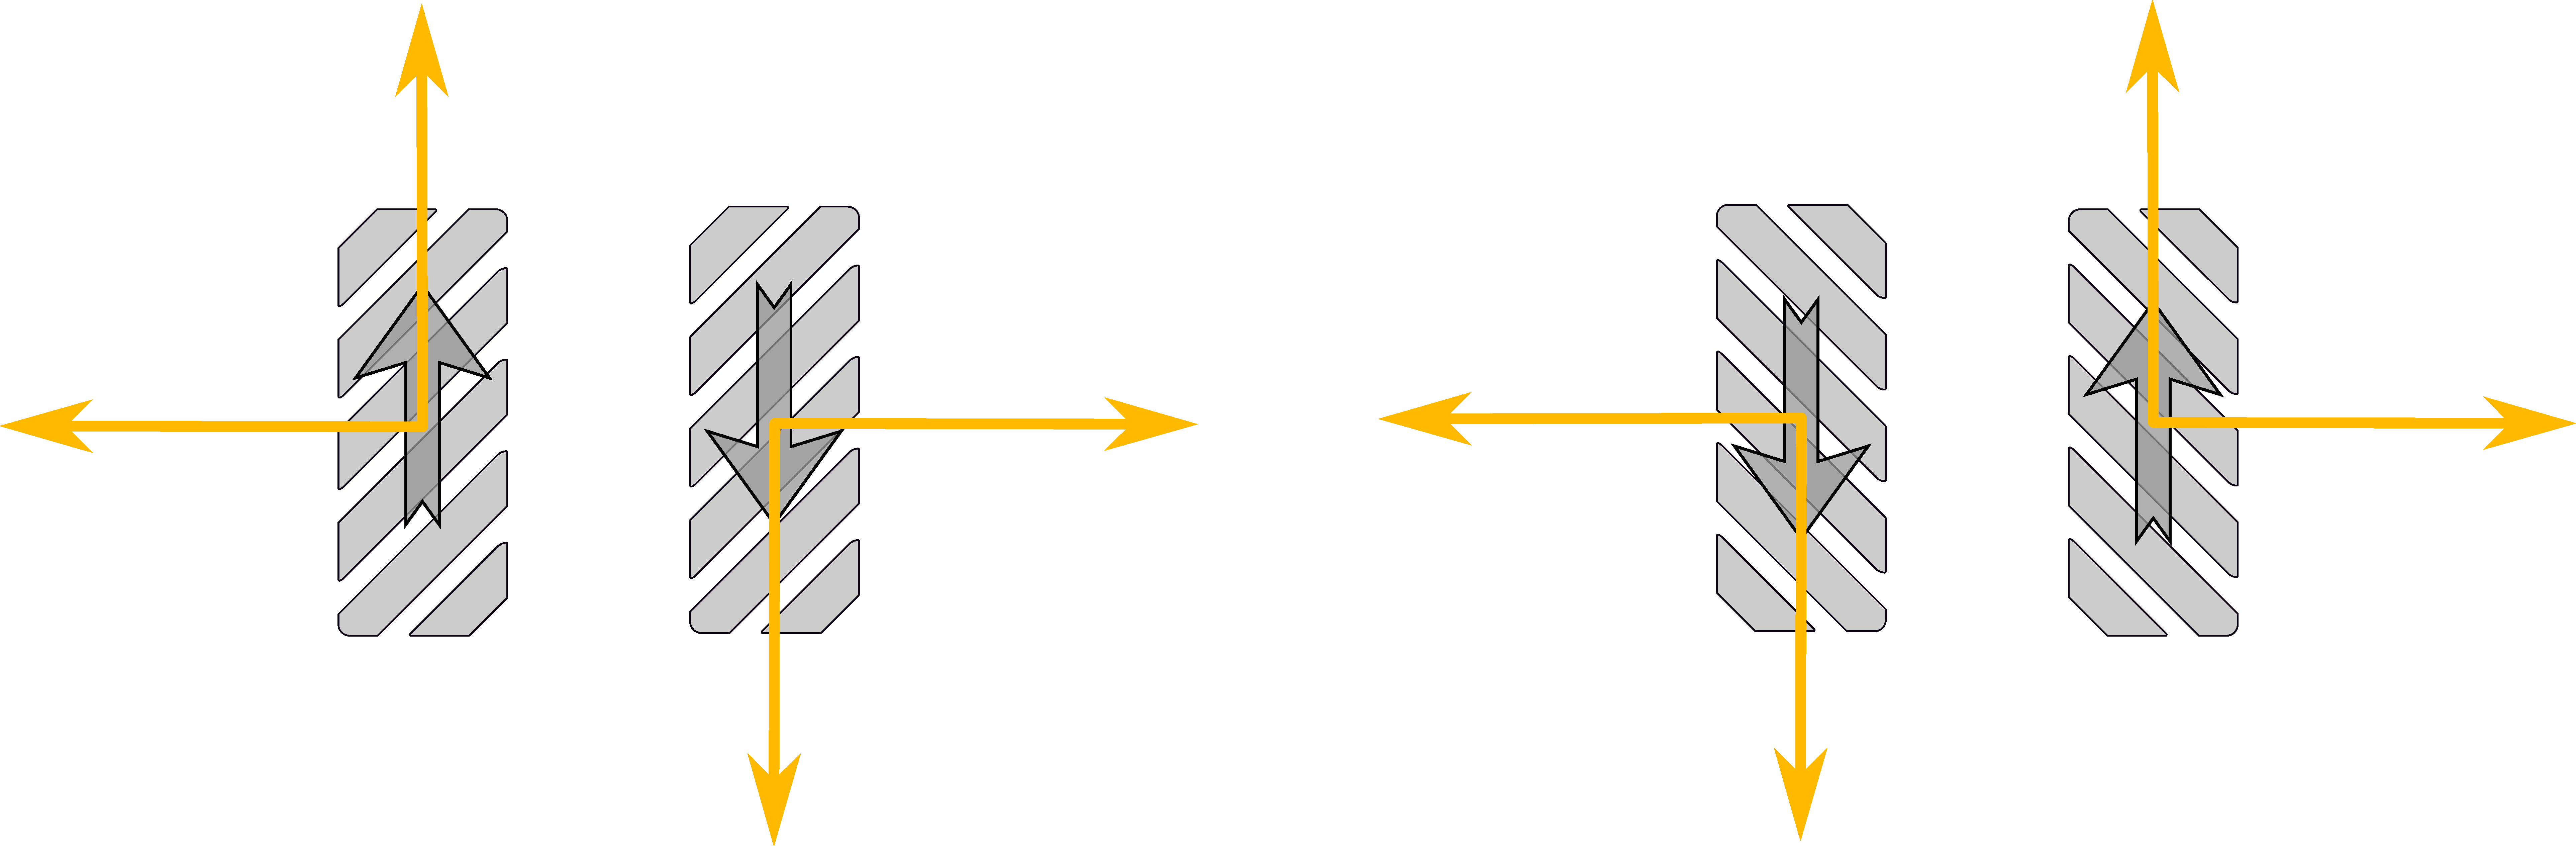
\includegraphics[width=\textwidth]{graphics/vectors.pdf}
			\caption{Wektory momentu siły i siły dla koła Mecanum, widzianego z góry.}
			\label{fig:wheel_vectors}
		\end{figure} 

		Ustawiając koła w odpowiedni sposób (rysunek \ref{fig:base_dims}), można wywołać odpowiednie znoszenie się wektorów sił,
		a w efekcie umożliwić platformie poruszanie się w kierunkach nieosiągalnych dla pojazdów o standardowych kołach.
		
		Można przedstawić te wektory na wcześniejszym rysunku \ref{fig:mecanum_dirs}.

		\begin{figure}[H]
			\centering
			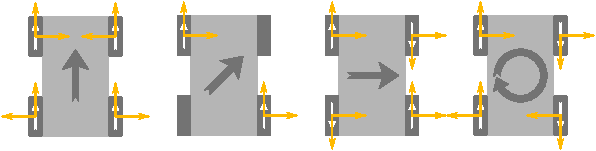
\includegraphics[width=\textwidth]{graphics/mecanum_dirs_vect.pdf}
			\caption{Ruchy platformy widzianej z góry, z nałożonymi składowymi wektorów sił.}
			\label{fig:mecanum_dirs_vect}
		\end{figure} 

		Należy wytłumaczyć podstawowe ruchy platformy. Kierunki osi są takie same, jak 
		opisane wcześniej (rysunek \ref{fig:base_ortho}).
		\begin{enumerate}
			\item Składowe wektorów sił w kierunku X znoszą się, ponieważ mają przeciwne zwroty na lewej i prawej parze kół.
			Pozostają jedynie składowe równoległe do osi Y, które powodują prostoliniowy ruch w tym kierunku.
			\item Dwa koła nie mają nadanego momentu siły. Wektory sił od pozostałych kół nadają platformie ruch pd kątem 45° do osi Y. 
			Warto zwrócić uwagę, że ruch odbywa się równolegle do kierunku $f_0$ dwóch zatrzymanych kół, zatem zgodnie z obrotem ich dolnych rolek, więc
			te koła nie powodują powstawania siły tarcia.
			\item Tutaj również składowe wektorów sił, równoległe do osi Y, znoszą się, podobnie jak w przypadku ruchu naprzód.
			Pozostają składowe równoległe do osi X, które nadają platformie przyspieszenie w bok.
			\item Prędkość kątowa wokół osi Z powstaje, gdy wypadkowa siła od kół po jednej stronie platformy znosi się z wypadkową siłą po drugiej stronie.
		\end{enumerate}

		Warto nadmienić, że w trakcie ruchu równolegle do osi Y, w idealnym przypadku rolki nie obracają się.
		Inaczej mówiąc, prędkość rolki będzie tym większa, im bardziej ruch koła wymuszany jest równolegle do osi koła.
		
		Przykładowo, przy ruchu w przód, rolki koła się nie obracają, lecz przy ruchu w bok ich prędkość obrotu jest znacznie większa.
		Ma to wpływ na zużywanie się tych elementów, nie tylko z punktu widzenia ilości obrotów danej rolki na pokonanym dystansie, 
		ale także sposobu w jaki wymuszany jest jej ruch.
		
		Rolki kół przy jeździe zawsze obracają się nieznacznie w obie strony, ze względu na nierówności powierzchni.
		Zatem przejazd przykładowego odcinka, przy platformie ustawionej przodem do kierunku jazdy, lub bokiem, będzie w różnym stopniu i w różny sposób zużywał elementy wykonawcze robota.
		To, jak dokładnie zużywają się przeguby i jaki styl jazdy opłaca się zastosować, aby zminimalizować uszkodzenia elementów jest dużą, odrębną dziedziną nauki.
		Odpowiednio skomplikowany algorytm sterowania może brać pod uwagę tą właściwość rolek.

\section{Enkodery}
	\label{sec:encoders}
	Silniki kół mają zamontowane enkodery. Czujniki te umożliwiają pomiar prędkości kątowej i kąta obrotu koła. 
	Korzystając z modelu kinematyki, można obliczyć z tych danych wypadkową prędkość robota, a następnie, za pomocą całkowania, wyznaczyć aktualną względną
	pozycję w stosunku do pozycji startowej.
	
\section{Silniki kół}
	\label{sec:motors}
	W opisywanym robocie, silniki kół są wstanie nadać im duży moment siły.
	To oznacza, że wartości prędkości kątowej kół, wykrytej przez enkodery, są zbliżone do prędkości zadanej.
	Ta właściwość jest potwierdzona testami (sekcja \ref{sec:test_velmobil}).
	Eksperymenty pokazały, że zasilacz robota ma ograniczony przesył prądu, więc jeśli silniki będą generowały zbyt duże momenty sił, może dojść do awaryjnego odłączenia się zasilacza, 
	co jest głównym powodem dla którego należy ograniczać nadawanie zbyt dużych przyspieszeń platformie.
	
\section{Skaner laserowy}
	\label{sec:lidar}
	Poślizg kół powoduje, że odometria, bazująca na danych generowanych przez enkodery, obarczona jest błędami losowymi i nie może być 
	użyta jako jedyna metoda wyznaczania pozycji względnej w trakcie jazdy robota \cite{heavy}.
	
	Dodatkowym czujnikiem, używanym do wyznaczania pozycji platformy, jest skaner laserowy.
	Platforma wyposażona jest w dwa czujniki typu LiDAR firmy SICK.
	LiDAR to zbitek wyrazów \emph{light} i \emph{radar}.

	\begin{figure}[h]
	\centering
	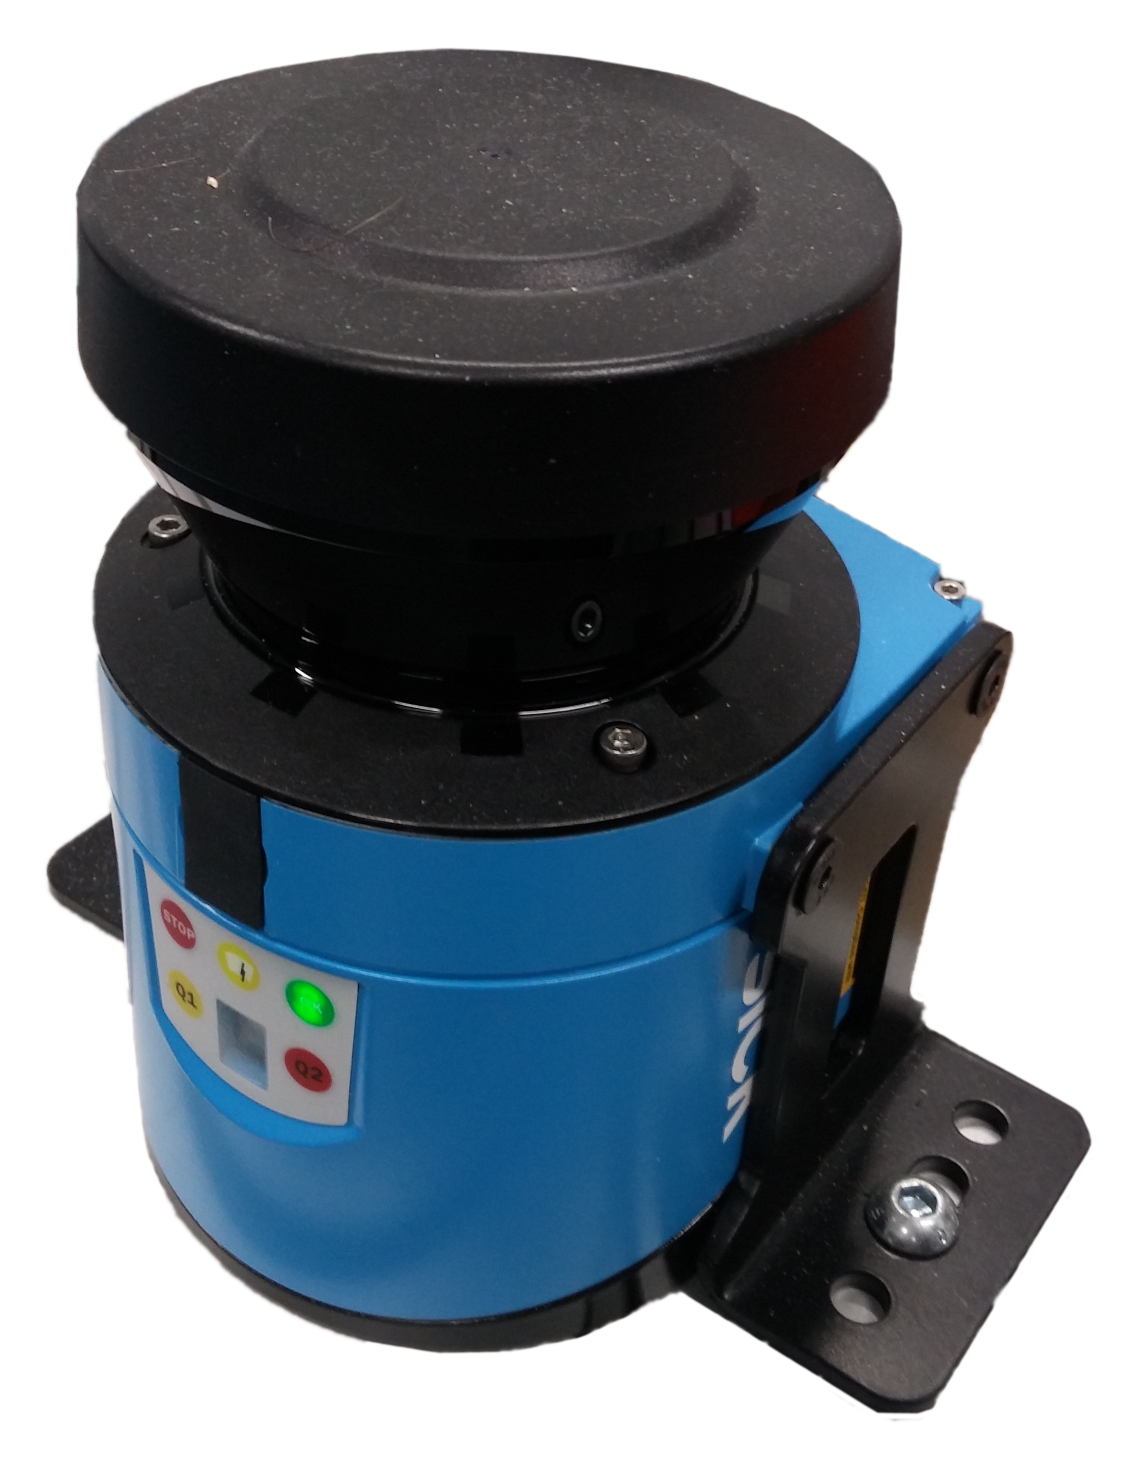
\includegraphics[width=0.5\textwidth]{graphics/sensor.png}
	\caption{Skaner laserowy SICK LMS100-10000.}
	\label{fig:sensor}
	\end{figure} 

	\subsection{Zasada działania}
		Wszystkie skanery tego typu mają bardzo podobną zasadę działania.
		W środku urządzenia znajduje się obrotowe lusterko, zwrócone pod kątem 45° do osi obrotu.
		Równolegle do osi jego obrotu znajduje się laser, który emituje impulsy z zakresie podczerwieni.
		Aktualna pozycja lusterka jest mierzona przez enkoder.
		Obok lasera jest czujnik, który bada odbite od obiektu światło.

		We wbudowanym mikrokontrolerze następuje pomiar czasu przelotu i natężenia światła.
		Na tej podstawie wyznaczana jest odległość obiektu od skanera.
		Skaner odpowiada także za usunięcie niektórych błędów pomiarowych i ewentualnych odbić promienia.
		Komunikacja z urządzeniem odbywa się po sieci Ethernet.

	\subsection{Podstawowe cechy}
		Czujnik składa się z dwóch części, głównego trzonu, oraz nakładki.
		Połączenie tych elementów powoduje, że jego zakres pomiaru posiada martwy kąt.
		Przedstawia to dobrze grafika producenta \ref{fig:lidar}.
		
		\begin{figure}[h]
			\centering
			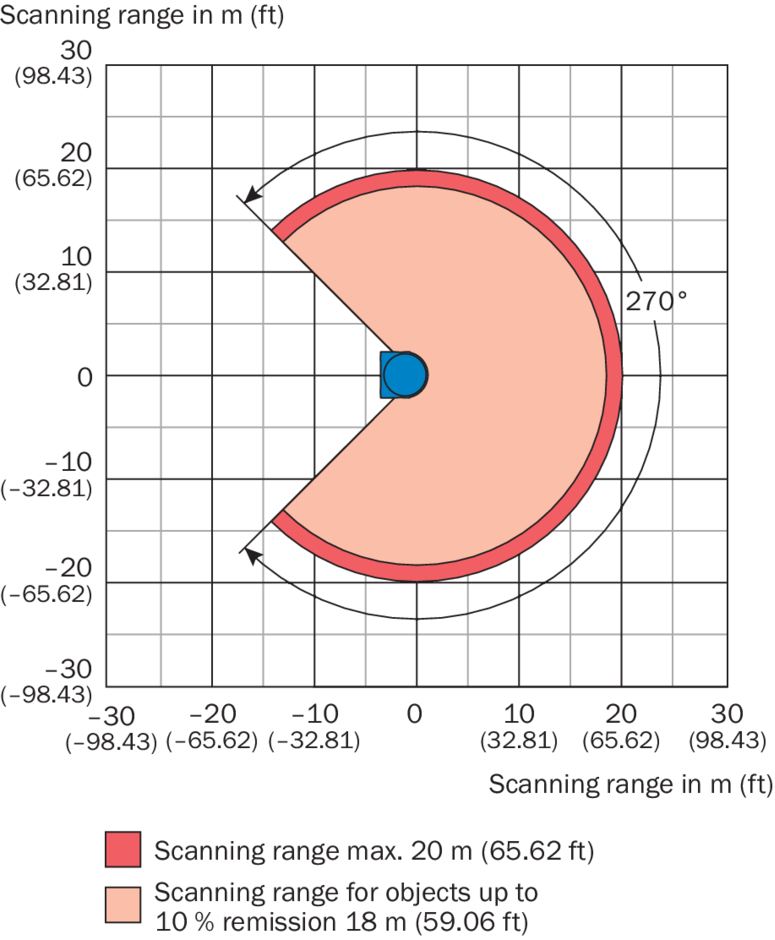
\includegraphics[width=0.6\textwidth]{graphics/sick.png}
			\caption{Wykres przedstawiający zasięg pomiarowy czujnika \cite{sick_website}.}
			\label{fig:lidar}
		\end{figure} 
		
		\begin{table}
			\centering
			\begin{tabular}{l r}
			Cecha & Wartość \\
			\hline
			Zakres kątowy pracy & \ang{270} \\
			Długość fali światła lasera & 905 \si{\nano\metre} (podczerwień) \\
			Częstotliwości skanowania & 25 \si{\hertz} / 50 \si{\hertz} \\
			Maksymalna odległość obiektu & $\approx$ 20 \si{\metre} \\
			Rozdzielczość kątowa & 0,25° / 0,5° \\
			Systematyczny błąd pomiarowy & $\pm$ 0,03 \si{\metre} \\
			Przypadkowy błąd pomiaru odległości & 0,012 \si{\metre} \\
			\end{tabular}
			\caption{Podstawowe cechy czujnika laserowego.}
			\label{tab:lidar}
		\end{table}
		
		Na podstawie danych z tabeli \ref{tab:lidar} można obliczyć, że w jednym przebiegu po całym zakresie kątowym urządzenia, 
		emitowane jest około 1080 lub 540 impulsów (w zależności od trybu działania).
		Taka liczba promieni wymagana jest w symulacji, aby wiernie odwzorować urządzenie.

\section{Jednostka inercyjna}
	Ten czujnik to małe urządzenie, posiadające zazwyczaj zestaw wewnętrznych czujników, przydatnych przy określaniu prędkości, orientacji i przyspieszeń modułu.
	Dodatkowo, wiele zestawów tego typu posiada także czujniki pola magnetycznego lub nawet termometry.
	
	Czujnik użyty w platformie to ADIS16460AMLZ, firmy Analog Devices \cite{adis_website}.
	Czujnik jest wyposażony w:
	\begin{itemize}
		\item Trzyosiowy żyroskop.
		\item Trzyosiowy akcelerometr.
		\item Czujnik temperatury.
		\item Sprzętowe wspomaganie korekcji błędów i kalibracji.
	\end{itemize}
	
	Błędy pomiarowe akcelerometra są bardzo duże, w stosunku do błędów pomiarowych żyroskopu i skanera laserowego. 
	Aby użyć tych danych w programie, należy zastosować algorytmy filtrujące szum i uśredniające wyniki.
	
	W symulacji nie jest używana informacja o temperaturze otoczenia, zatem nie ma potrzeby jej symulować.
	
\section{Sterowanie urządzeniami}
	Urządzenia robota przyjmują sterowanie w formie odpowiednich dla siebie pakietów sieciowych.
	Struktury wiadomości, używane w komunikacji w ROSie, nie mogą być bezpośrednio użyte do sterowania sprzętowego.
	W tym celu platforma podłączona jest do specjalnego komputera, pracującego z systemem operacyjnym czasu rzeczywistego, który to odpowiada za bezpośrednią komunikację
	z platformą.
	
	Komendy dla robota w formie pakietów sieciowych, zawierających bezpośrednie wiadomości środowiska ROS, są nadawane poprzez sieć do tego pośrednika, który na ich podstawie odpowiednio obsługuje urządzenia. Możliwe jest także odbieranie pomiarów z czujników w podobny sposób.
	
